\documentclass[11pt]{article}
\usepackage[english]{babel}
\usepackage[utf8x]{inputenc}
\usepackage{amsmath}
\usepackage{graphicx}
\usepackage[colorinlistoftodos]{todonotes}
\usepackage{listings}
\usepackage[hmargin=2cm]{geometry}
\usepackage{color} 
\definecolor{codegreen}{rgb}{0,0.6,0}
\definecolor{codegray}{rgb}{0.5,0.5,0.5}
\definecolor{codepurple}{rgb}{0.58,0,0.82}
\definecolor{backcolour}{rgb}{0.95,0.95,0.92} 
\lstdefinestyle{mystyle}{
    backgroundcolor=\color{backcolour},   
    commentstyle=\color{codegreen},
    keywordstyle=\color{magenta},
    numberstyle=\tiny\color{blue},
    stringstyle=\color{codepurple},
    basicstyle=\footnotesize,
    breakatwhitespace=false,         
    breaklines=true,                 
    captionpos=b,                    
    keepspaces=true,                 
    numbers=left,                    
    numbersep=5pt,                  
    showspaces=false,                
    showstringspaces=false,
    showtabs=false,                  
    tabsize=2
}
\lstset{style=mystyle}
\begin{document}
\begin{titlepage}
\newcommand{\HRule}{\rule{\linewidth}{0.5mm}}
\center
\textsc{\LARGE Universidad de Granada}\\[1.5cm] % Name of your university/college
\textsc{\Large Algorítmica}\\[0.5cm] % Major heading such as course name
\textsc{\large Memoria de Prácticas}\\[0.5cm] % Minor heading such as course title
\HRule \\[0.4cm]
{ \huge \bfseries Práctica IV: Backtracking}\\[0.4cm] % Title of your document
\HRule \\[1.5cm]
\begin{minipage}{0.4\textwidth}
\begin{flushleft} \large
\emph{Autor:}\\
Antonio Gámiz Delgado\textsc{} % Your name
\end{flushleft}
\end{minipage}
~
\begin{minipage}{0.4\textwidth}
\begin{flushright} \large
\emph{} \\
\textsc{} % Supervisor's Name
\end{flushright}
\end{minipage}\\[2cm]
{\large \today}\\[2cm] % Date, change the \today to a set date if you want to be precise

\includegraphics{logo.png}\\[1cm]
\vfill % Fill the rest of the page with whitespace
\end{titlepage}

\section{Problema}

Se va a celebrar una cene de gala a la que asistirán $n$ invitados. Todos se van a sentar alrededor de una única gran mesa rectangular, de forma que cada invitado tendrá sentados junto a él a otros dos comensales (uno a su izquierda y otro a su derecha). En función de las característiscas de cada invitado (por ejemplo po categoría, puesto, lugar de procedencia...) existen unas normas de protocolo que indican el nivel de conveniencia de que dos invitados se siente en lugares contiguos (supondremos que dicho nivel es un número entero entre 0 y 100). El nivel de conveniencia total de una asignación de invitados a su puesto en la mesa es la suma de todos los niveles de conveniencia de cada invitado con cada uno de los dos invitados sentados a su lado.

Se desea sentar a los invitados de forma que el nivel de conveniencia global sea lo mayor posible. Diseñar e implementar un algoritmo vuelta atrás para resolver este problema. Realizar un estudio empírico de su eficiencia.

\section{Representación de la conveniencia}

Para implementar la conveniencia, he creado una clase independiente llamada $ConvenienceMatrix$ para obtener mayor generalidad a la hora de representarla (en caso de que queramos modificar como se obtiene la conveniencia solo tenemos que modificar esa clase y no el algoritmo entero).

Además también he aprovechado para añadirle a esa clase un método que calcule el costo de una solución dada algunos métodos útiles para el algoritmo, como:

\section{Diseño del algoritmo backtracking}

Para resolver el problema, primero empecé a desorrar la implementación de un árbol para luego rellenarlo, podarlo, etc, pero luego me di cuenta que con una función recursiva bastante simple obteníamos el mismo resultado saltándonos la complejidad que acarrea un árbol general.

Por lo que, a continuación expongo el algoritmo en sí y algunas variables globales que he usado (no es buena práctica usar variables globales, pero debido a que simplifican el diseño y aportar claridad he visto conveniente usarlas en esta código).

\begin{lstlisting}[language=C++, caption=Algoritmo backtracking]
void backtracking(ConvenienceMatrix & c, vector<int> v)
{
	vector<int> available=supplementary(v, c.size()); //definida en 'auxliar.cpp'
	for(int i=0; i<available.size(); i++)
	{
	v.push_back(available[i]); //aniadimos el siguiente numero que no este ya en la solucion
	if( v.size() == c.size() ) ++count;//to_s(v); //descomentar para ver todas las posibilidades
	aux_cost=c.costs(v);
	if(aux_cost > cost) //guardamos la solucion con el mayor coste
	{
		cost=aux_cost;
		solution=v;
		backtracking(c, v);
	}
	
	if(v.size()<7) backtracking(c, v); //recursividad
	
	v.pop_back(); //eliminamos el elemento aniadido antes para calcular
				  //la siguiente posibilidad
	}
}
\end{lstlisting}

Con esta función recursiva lo que hacemos es calcular todas las permutaciones sin repeteción de los $n-1$ números (los asistentes a la cena de gala los númeramos desde $0$ hasta $n-1$). Para calcular todas esas posibilidades, he usado la función $vector<int> supplementary(vector<int> \& v)$:

\begin{lstlisting}[language=C++, caption=función auxiliar]
//supplementary of v respect to [0...n-1]
vector<int> supplementary(vector<int> & v, int n)
{
	vector<int> result;
	for(int i=0; i<n; i++) if( !is_in(v, i) ) result.push_back(i);
	return result;
}
\end{lstlisting}

Que como su nombre indica, calcula el complementario un vector de enteros dado con respecto al vector que contiene los enteros desde $0$ hasta $n-1$.

El resultado de $supplementary$ son los enteros que faltan por contemplar en la solución, por lo que una vez calculado, llamamos otra vez a la función, con el mismo vector $v$, pero en cada iteración le añadimos un elemento de los que le falta, obteniendo así todas las posibilidades.

Además he declarado las siguientes variables globales para calcular el máximo:

\begin{lstlisting}[language=C++, caption=Variables globales]
static int count = 0; //numero de soluciones calculadas
vector<int> solution; //mejor solucuion
int cost; //coste de la solucion
int aux_cost; //coste auxiliar para calcular el maximo
\end{lstlisting}

Para ahorrarme calcular todas las posibilidades, calculo todas las posibilidades hasta que tengan longitud 7, después de eso, solo desarrollo las que tengan costo más grande, que son las que buscamos.

\section{Eficiencia empírica}

Para calcular la eficiencia empírica he hecho un script en python (llamado $script.py$) para ejecutar el programa con un tamaño $n$ desde 1 hasta 11.

Además de la función descrita anteriormente, también he probado empíricamente otras dos variaciones de la misma:

En esta variación de la función desarrallomas todas las soluciones "$peores$" que la que tenemos actualmente. Parece un poco raro, pero al final llega a una solución óptima descartando algunos casos (menos de los deseados, se verá después en la representación).

\begin{lstlisting}[language=C++, caption=Variación 1]
void backtracking(ConvenienceMatrix & c, vector<int> v)
{
	vector<int> available=supplementary(v, c.size()); //definida en 'auxliar.cpp'
	for(int i=0; i<available.size(); i++)
	{
	v.push_back(available[i] ); //aniadimos el siguiente numero que no este ya en la solucion
	if( v.size() == c.size() ) ++count;//to_s(v); //descomentar para ver todas las posibilidades
	aux_cost=c.costs(v);
	if(aux_cost > cost  ) //guardamos la solucion con el mayor coste
	{
		cost=aux_cost;
		solution=v;
	}
	
	else backtracking(c, v); //recursividad
	
	v.pop_back(); //eliminamos el elemento aniadido antes para calcular
	//la siguiente posibilidad
	}
}
\end{lstlisting}

Esta variación hace que el algoritmo no sea $backtracking$, es decir, esta versión contempla las $n!$ posibilidades y escoge la mejor. La he añadido para ver la mejora respecto a usar backtracking o no.

\begin{lstlisting}[language=C++, caption=Variación 2]
void backtracking(ConvenienceMatrix & c, vector<int> v)
{
	vector<int> available=supplementary(v, c.size()); //definida en 'auxliar.cpp'
	for(int i=0; i<available.size(); i++)
	{
	v.push_back(available[i] ); //aniadimos el siguiente numero que no este ya en la solucion
	if( v.size() == c.size() ) ++count;//to_s(v); //descomentar para ver todas las posibilidades
	aux_cost=c.costs(v);
	if(aux_cost > cost  ) //guardamos la solucion con el mayor coste
	{
		cost=aux_cost;
		solution=v;
	}
	
	backtracking(c, v); //recursividad
	
	v.pop_back(); //eliminamos el elemento aniadido antes para calcular
	//la siguiente posibilidad
	}
}

\end{lstlisting}

A continuación veremos las representaciones gráficas por separado de cada una de las variaciones del algoritmo, y luego las veremos conjuntamente para ver la diferencia.

\begin{figure}[h]
	\centering
	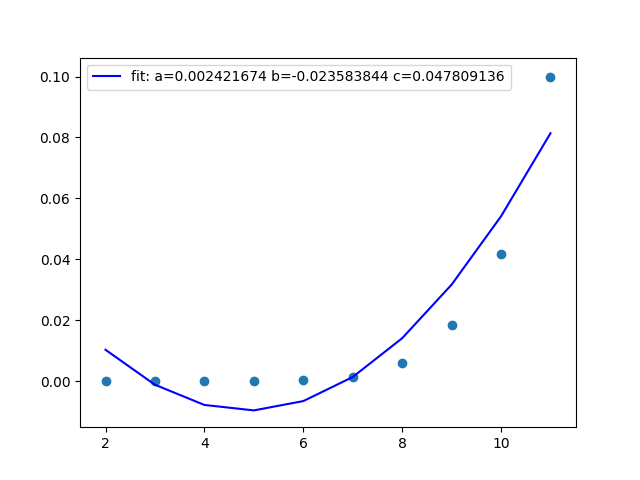
\includegraphics[scale=0.5]{../graphics/metodo1.png}
	\caption{Eficiencia Empírica Método 1}
	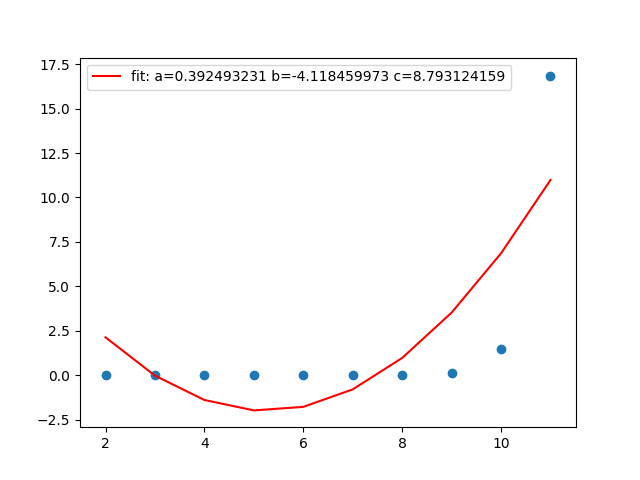
\includegraphics[scale=0.5]{../graphics/metodo2.png}
	\caption{Eficiencia Empírica Método 2}
	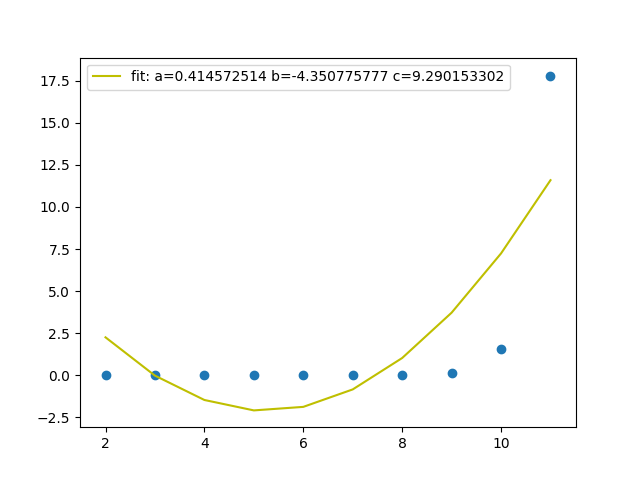
\includegraphics[scale=0.5]{../graphics/metodo3.png}
	\caption{Eficiencia Empírica Método 3}
\end{figure}

En las gráficas podemos ver que los puntos, hacia el tamaño $n=11$, dan un salta muy brusco, esto se debe a que la eficiencia del algoritmo a lo bruto es de orden $O(n!)$.

Además, vemos que la diferencia entre el algoritmo a lo bruto (3), y la variación 2 (2), es muy pequeña (aunque para $n$ lo suficientemente grande la diferencia es considerable). Esto se debe a que la condición que tiene cumplir el algoritmo (2) para desarrollar más soluciones, se cumple para muchos casos.

En cambio, vemos que el tiempo del algoritmo (1) es mucho menor. Esto se debe a que solo desarrollamos los primeros 7 niveles iniciales de las soluciones, después de eso, aplicamos backtracking y solo desarrollamos las soluciones con mayor costo. Aunque ganamos mucho en eficiencia, la solución no es la mejor (como pasa siempre en (2) y bastante frecuentemente con (3).

\begin{figure}[h]
	\centering
	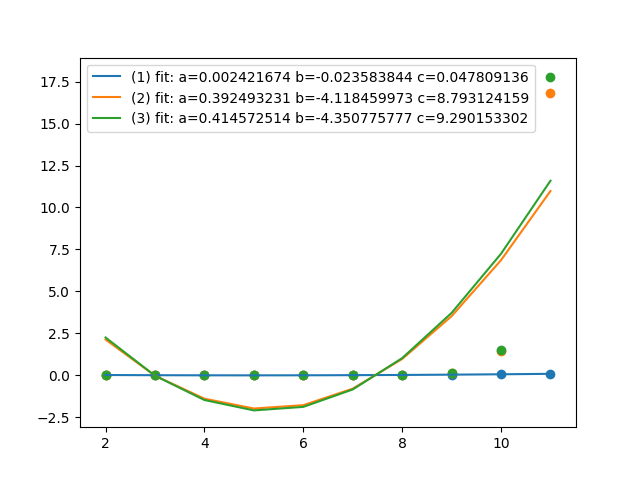
\includegraphics[scale=0.6]{../graphics/juntas.png}
	\caption{Eficiencia Empírica General}
\end{figure}


\end{document}